%!TEX root = ../main.tex

\chapter{Machine Learning}\label{cha:machinelearning}

In this chapter a new approach to identifying strategies that are the same will be presented.
A new type of tournament will be presented, and the summary of the results of this tournament will then be used to train a Machine Learning model.
The model is then able to predict whether new strategies are the same as ones already implemented within Axelrod-Python.

\section{Ashlock Tournament}\label{sec:ashlock_tourn}
In an Ashlock tournament, all strategies entered play against a probe strategy for a range of parameters, and do not play each other.
A results file is then created with information about how the strategies performed and behaved in the tournament.

\begin{sidewaystable}[htbp!]
\begin{tabular}{llllllllllHHH}
\toprule
Name &  Median\_score &  Cooperation\_rating &  Wins &  Initial\_C\_rate &  CC\_rate &  CD\_rate &  DC\_rate &  DD\_rate &  CC\_to\_C\_rate &  CD\_to\_C\_rate &  DC\_to\_C\_rate &  DD\_to\_C\_rate \\
\midrule
Defector & 0.59536 & 0.0000 & 22.0 & 0.0 & 0.0000 & 0.0000 & 0.4942 & 0.5058 & 0.0 & 0.0 & 0.0 & 0.0 \\
Win-Stay Lose-Shift & 0.46868 & 0.5528 & 7.0 & 1.0 & 0.3302 & 0.2226 & 0.2264 & 0.2208 & 1.0 & 0.0 & 0.0 &           1.0 \\
Bully & 0.46388 & 0.5024 & 11.0 & 0.0 & 0.1606 & 0.3418 & 0.3350 & 0.1626 & 0.0 & 1.0 & 0.0 & 1.0 \\
Alternator & 0.44824 & 0.5000 &  13.0 & 1.0 & 0.2484 & 0.2516 & 0.2490 & 0.2510 & 0.0 & 0.0 & 1.0 & 1.0 \\
 Tit For Tat & 0.43360 & 0.5144 & 0.0 & 1.0 & 0.3680 & 0.1464 & 0.1446 & 0.3410 & 1.0 & 0.0 & 1.0 & 0.0 \\
\bottomrule
\end{tabular}

\begin{tabular}{lHHHHHHHHHlll}
\toprule
Name &  Median\_score &  Cooperation\_rating &  Wins &  Initial\_C\_rate &  CC\_rate &  CD\_rate &  DC\_rate &  DD\_rate &  CC\_to\_C\_rate &  CD\_to\_C\_rate &  DC\_to\_C\_rate &  DD\_to\_C\_rate \\
\midrule
Defector & 0.59536 & 0.0000 & 22.0 & 0.0 & 0.0000 & 0.0000 & 0.4942 & 0.5058 & 0.0 & 0.0 & 0.0 & 0.0 \\
Win-Stay Lose-Shift & 0.46868 & 0.5528 & 7.0 & 1.0 & 0.3302 & 0.2226 & 0.2264 & 0.2208 & 1.0 & 0.0 & 0.0 &           1.0 \\
Bully & 0.46388 & 0.5024 & 11.0 & 0.0 & 0.1606 & 0.3418 & 0.3350 & 0.1626 & 0.0 & 1.0 & 0.0 & 1.0 \\
Alternator & 0.44824 & 0.5000 &  13.0 & 1.0 & 0.2484 & 0.2516 & 0.2490 & 0.2510 & 0.0 & 0.0 & 1.0 & 1.0 \\
 Tit For Tat & 0.43360 & 0.5144 & 0.0 & 1.0 & 0.3680 & 0.1464 & 0.1446 & 0.3410 & 1.0 & 0.0 & 1.0 & 0.0 \\
\bottomrule
\end{tabular}
\caption{table 1}

\bigskip

\begin{tabular}{lllllllllHHHHH}
\toprule
Name\_A & Name\_B & Median\_score\_r & Cooperation\_rating\_r & Wins\_r & Initial\_C\_rate\_r & CC\_rate\_r & CD\_rate\_r & DC\_rate\_r & DD\_rate\_r & CC\_to\_C\_rate\_r & CD\_to\_C\_rate\_r & DC\_to\_C\_rate\_r & DD\_to\_C\_rate\_r \\
\midrule
 Defector & Defector & 1.000000 & 1.0 &  1.000000 & 1.0 & 1.0 & 1.0 & 1.000000 & 1.000000 & 1.0 & 1.0 & 1.0 & 1.0 \\
 Defector & Win-Stay Lose-Shift &0.787221 & 0.0 &  0.318182 & 0.0 & 0.0 & 0.0 & 0.458114 & 0.436536 & 0.0 & 1.0 & 1.0 & 0.0 \\
 Defector & Bully & 0.779159 & 0.0 & 0.500000 & 1.0 & 0.0 & 0.0 & 0.677863 & 0.321471 & 1.0 & 0.0 & 1.0 & 0.0 \\
 Defector & Alternator & 0.752889 & 0.0 & 0.590909 & 0.0 & 0.0 & 0.0 & 0.503845 & 0.496244 & 1.0 & 1.0 & 0.0 & 0.0 \\
 Defector & Tit For Tat & 0.728299 & 0.0 &  0.000000 & 0.0 & 0.0 & 0.0 & 0.292594 & 0.674180 & 0.0 & 1.0 & 0.0 & 1.0 \\
\bottomrule
\end{tabular}
\begin{tabular}{llHHHHHHHHllll}
\toprule
Name\_A & Name\_B & Median\_score\_r & Cooperation\_rating\_r & Wins\_r & Initial\_C\_rate\_r & CC\_rate\_r & CD\_rate\_r & DC\_rate\_r & DD\_rate\_r & CC\_to\_C\_rate\_r & CD\_to\_C\_rate\_r & DC\_to\_C\_rate\_r & DD\_to\_C\_rate\_r \\
\midrule
 Defector & Defector & 1.000000 & 1.0 &  1.000000 & 1.0 & 1.0 & 1.0 & 1.000000 & 1.000000 & 1.0 & 1.0 & 1.0 & 1.0 \\
 Defector & Win-Stay Lose-Shift &0.787221 & 0.0 &  0.318182 & 0.0 & 0.0 & 0.0 & 0.458114 & 0.436536 & 0.0 & 1.0 & 1.0 & 0.0 \\
 Defector & Bully & 0.779159 & 0.0 & 0.500000 & 1.0 & 0.0 & 0.0 & 0.677863 & 0.321471 & 1.0 & 0.0 & 1.0 & 0.0 \\
 Defector & Alternator & 0.752889 & 0.0 & 0.590909 & 0.0 & 0.0 & 0.0 & 0.503845 & 0.496244 & 1.0 & 1.0 & 0.0 & 0.0 \\
 Defector & Tit For Tat & 0.728299 & 0.0 &  0.000000 & 0.0 & 0.0 & 0.0 & 0.292594 & 0.674180 & 0.0 & 1.0 & 0.0 & 1.0 \\
\bottomrule
\end{tabular}
\caption{table 2}
\end{sidewaystable}



\section{Training the model}\label{sec:training_model}

To train the model, all strategies available in Axelrod-Python were entered into an Ashlock tournament.
T

A new table can then be produced where the results of each strategies are compared.
Given two strategies $A$ and $B$, they have a set of variables $\{x_1^{(A)}, x_2^{(A)}, \dots, x_n^{(A)}\}$ or $\{x_1^{(B)}, x_2^{(B)}, \dots, x_n^{(B)}\}$ which are taken from the results file.
To compare the strategies, a new set of variables $\{r_1, r_2, \dots, r_n \}$ is created where:
$$
r_k = \frac{\min(x_k^{(A)}, x_k^{(B)})}{\max(x_k^{(A)}, x_k^{(B)})}.
$$
In the case where $x_k^{(A)} = x_k^{(B)} = 0$, the ratio $r_k$ is set to 1 as the two variables are equal.
By comparing the names of the two strategies, a new column can be added to the data containing a boolean variable where a value of 1 implies that the two strategies are the same, and 0 if they are different.


\section{Initial Results}

\begin{figure}[htbp!]
    \centering
    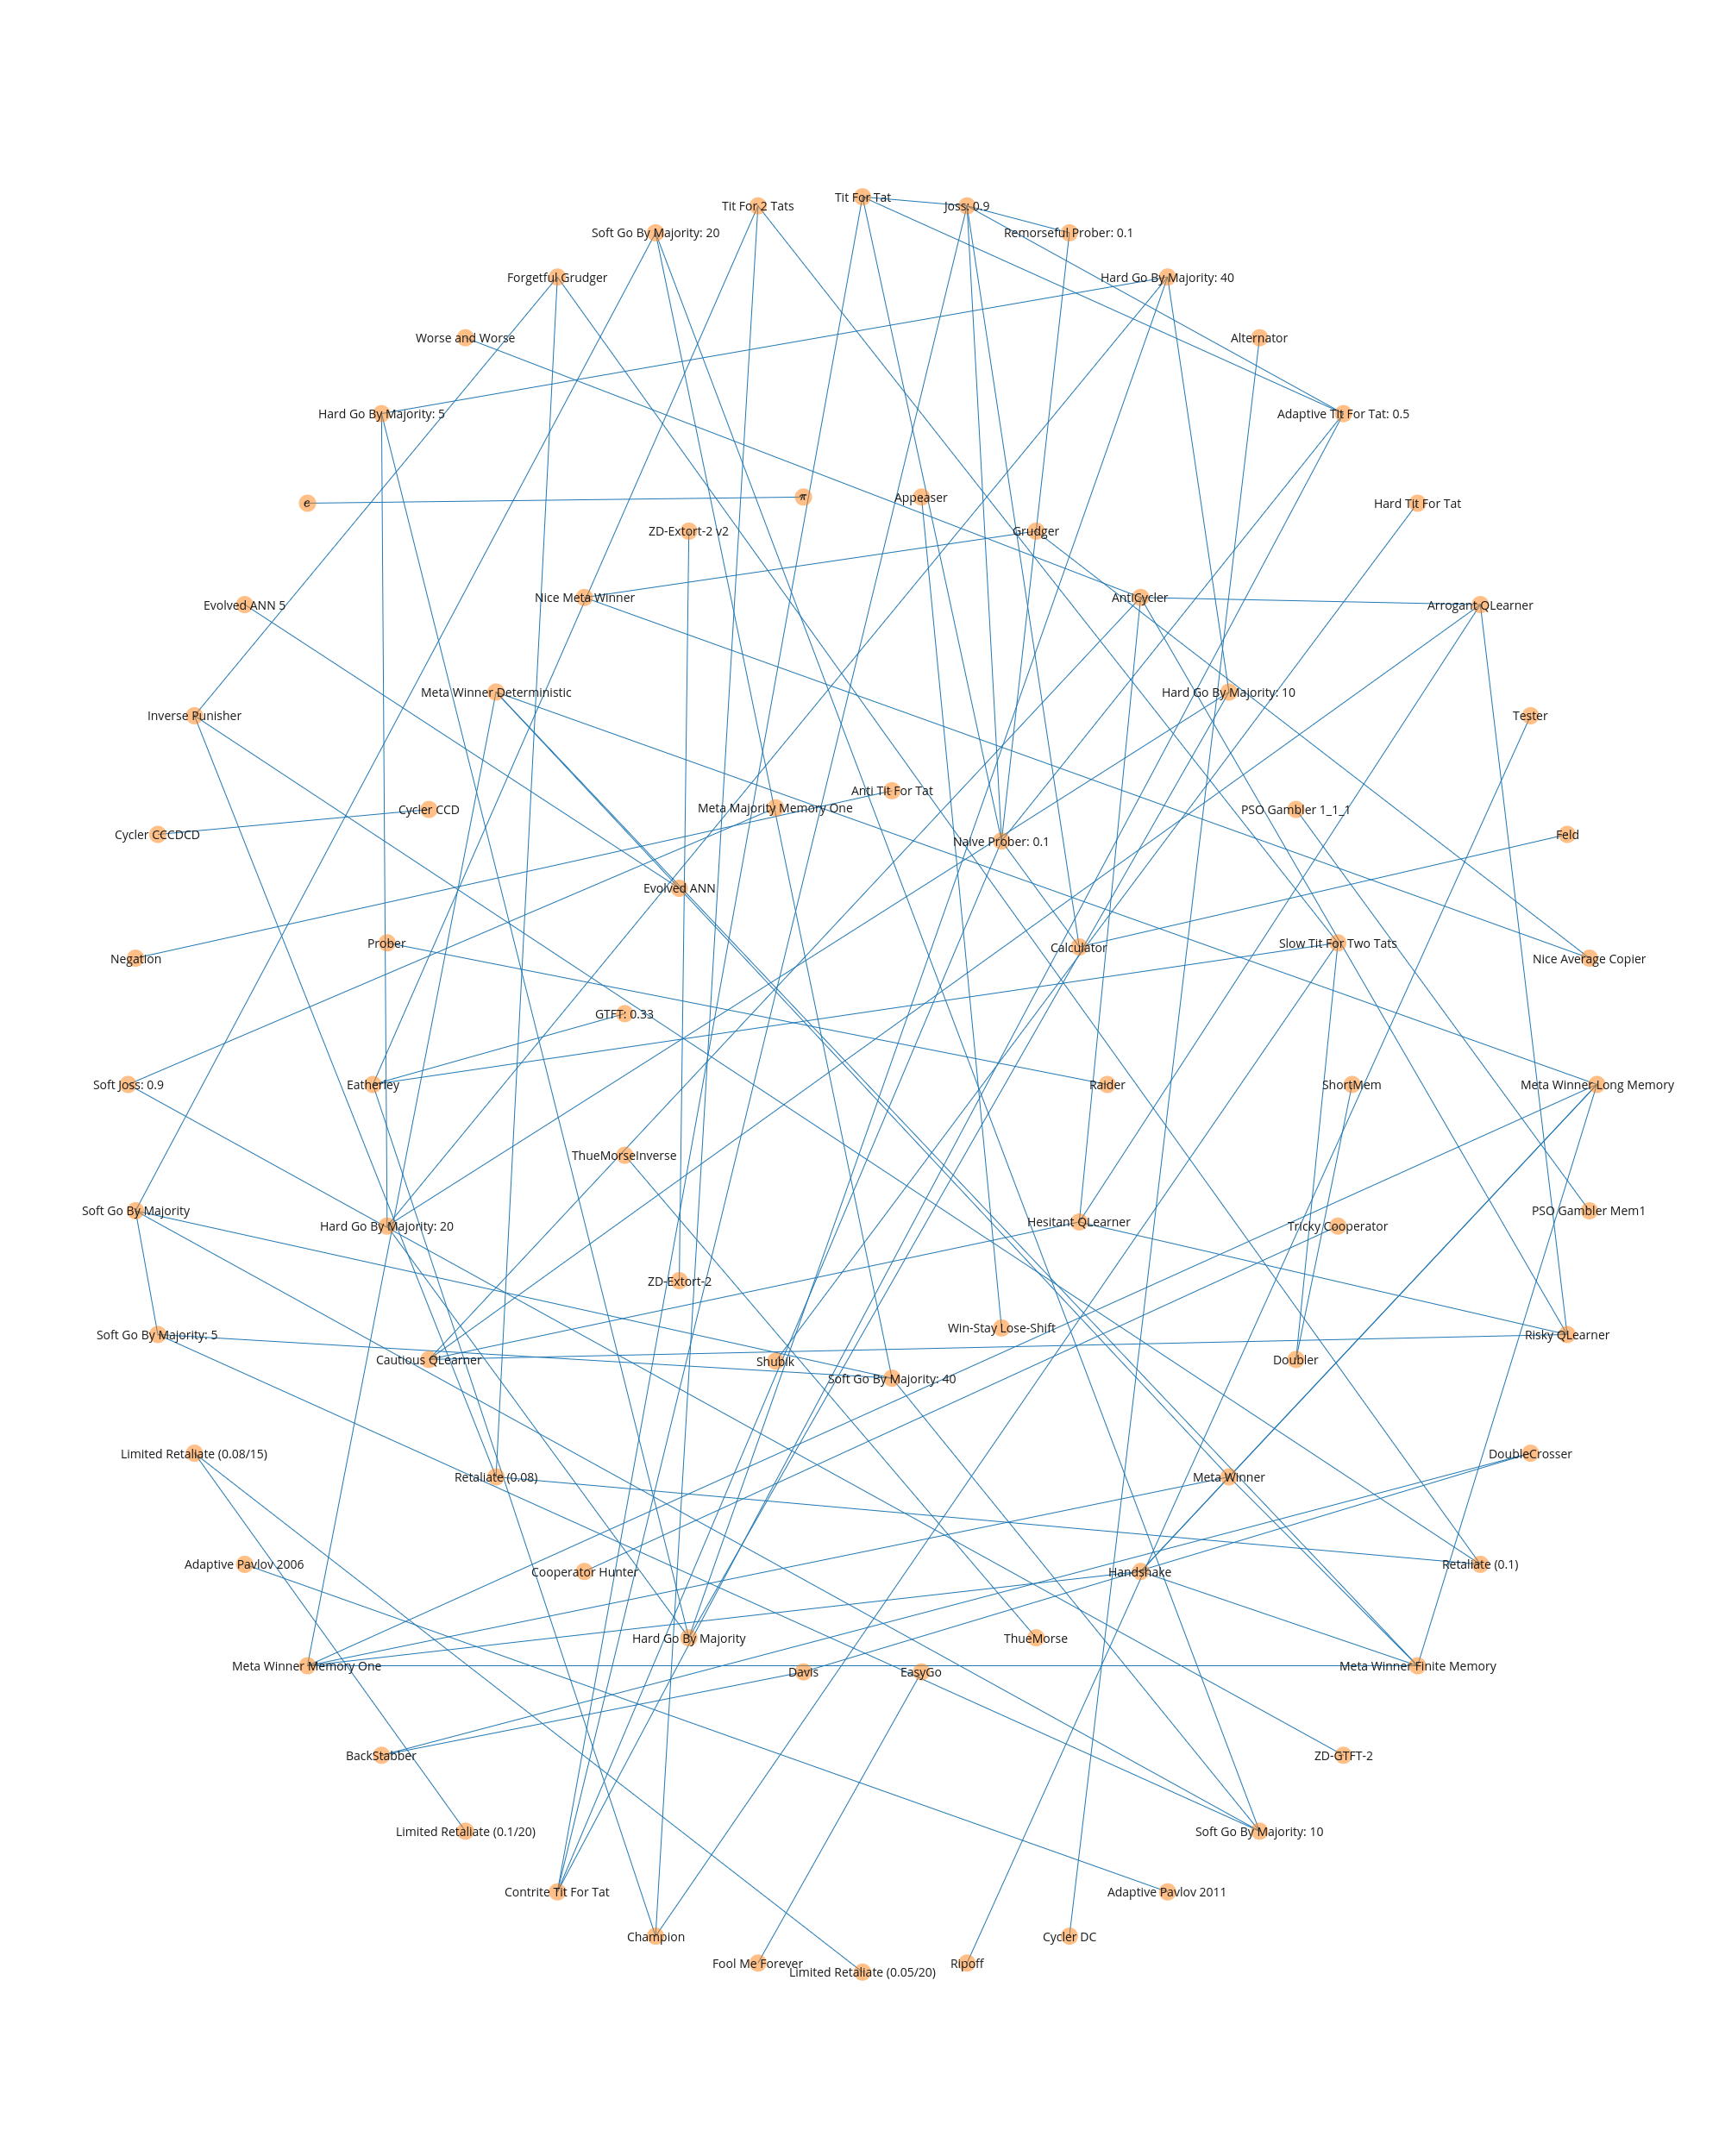
\includegraphics[width=\linewidth]{../img/neighbourhoods/overall.png}
    \caption{Caption here}
    \label{fig:figure1}
\end{figure}

% \begin{figure}[htbp!]
% \subfloat[]{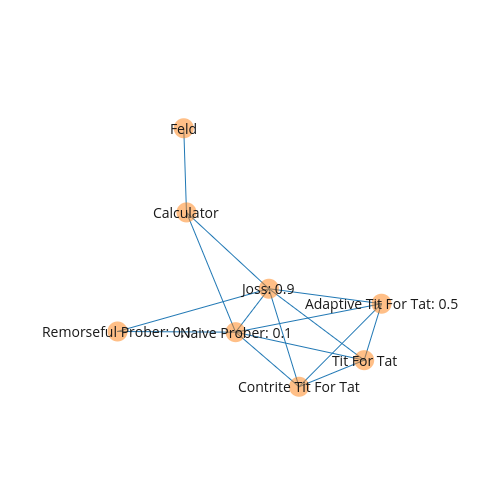
\includegraphics[width = 0.3\textwidth]{../img/neighbourhoods/1.png}}
% \subfloat[]{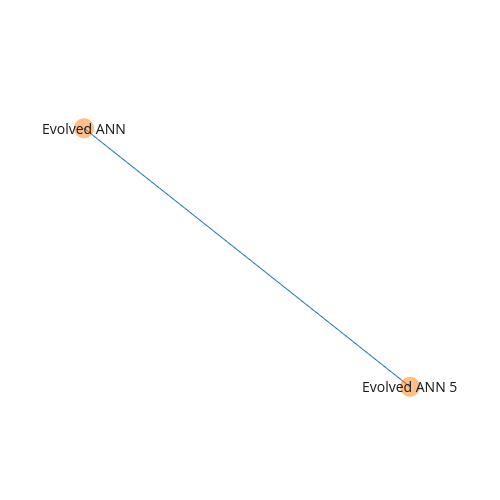
\includegraphics[width = 0.3\textwidth]{../img/neighbourhoods/2.png}}
% \subfloat[]{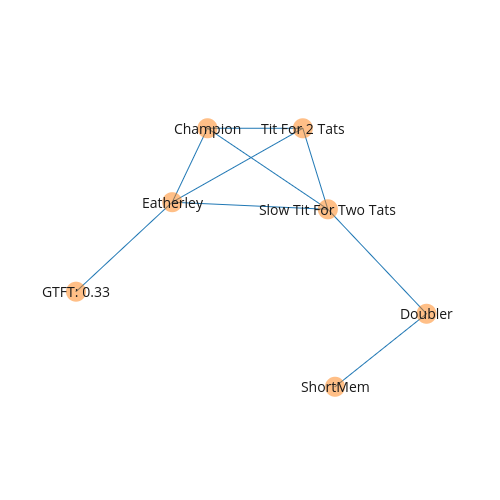
\includegraphics[width = 0.3\textwidth]{../img/neighbourhoods/3.png}} \\
% \end{figure}
% \begin{figure}[htbp!]
% \ContinuedFloat
% \subfloat[]{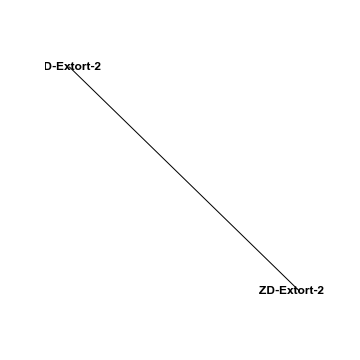
\includegraphics[width = 0.3\textwidth]{../img/neighbourhoods/4.png}}
% \subfloat[]{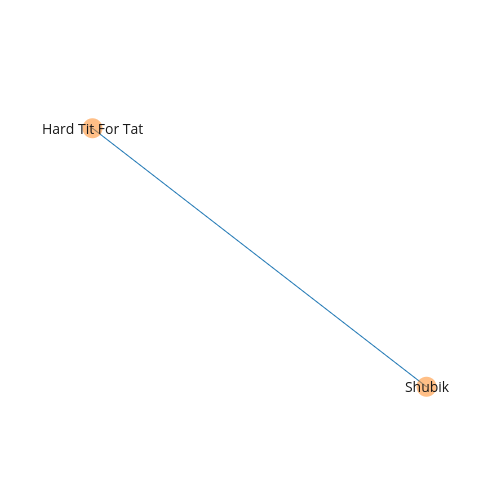
\includegraphics[width = 0.3\textwidth]{../img/neighbourhoods/5.png}}
% \subfloat[]{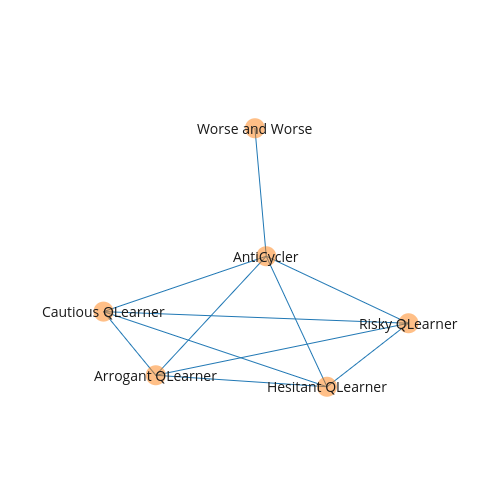
\includegraphics[width = 0.3\textwidth]{../img/neighbourhoods/6.png}} \\
% \end{figure}
% \begin{figure}[htbp!]
% \ContinuedFloat
% \subfloat[]{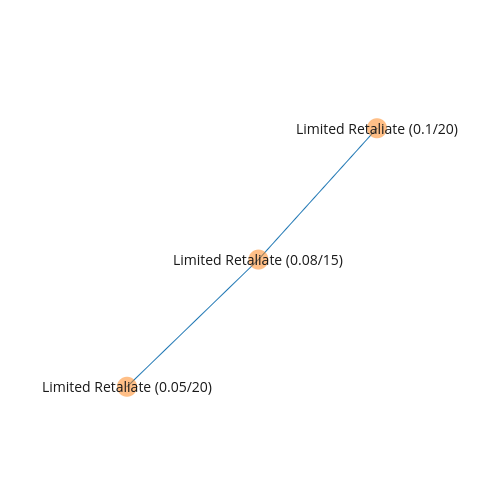
\includegraphics[width = 0.3\textwidth]{../img/neighbourhoods/7.png}}
% \subfloat[]{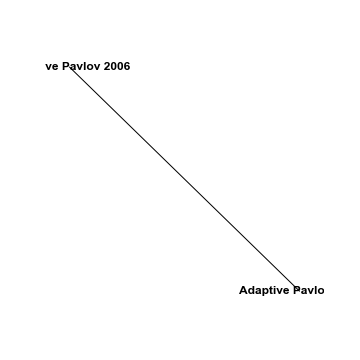
\includegraphics[width = 0.3\textwidth]{../img/neighbourhoods/8.png}}
% \subfloat[]{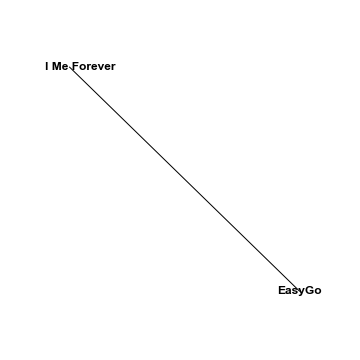
\includegraphics[width = 0.3\textwidth]{../img/neighbourhoods/9.png}} \\
% \end{figure}
% \begin{figure}[htbp!]
% \ContinuedFloat
% \subfloat[]{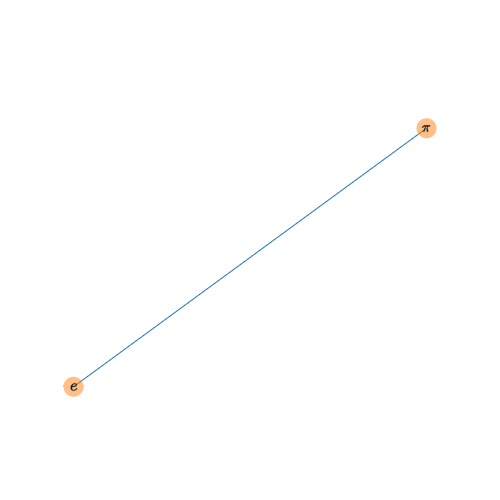
\includegraphics[width = 0.3\textwidth]{../img/neighbourhoods/10.png}}
% \subfloat[]{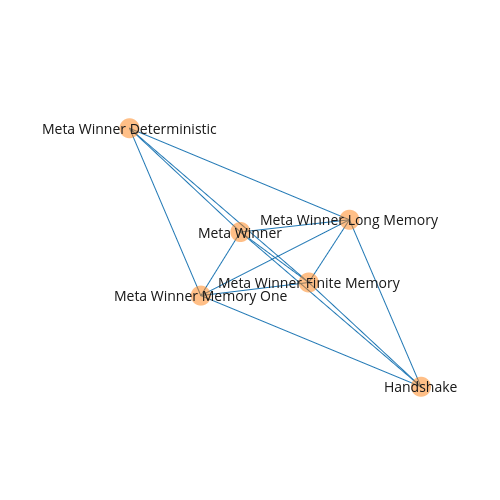
\includegraphics[width = 0.3\textwidth]{../img/neighbourhoods/11.png}}
% \subfloat[]{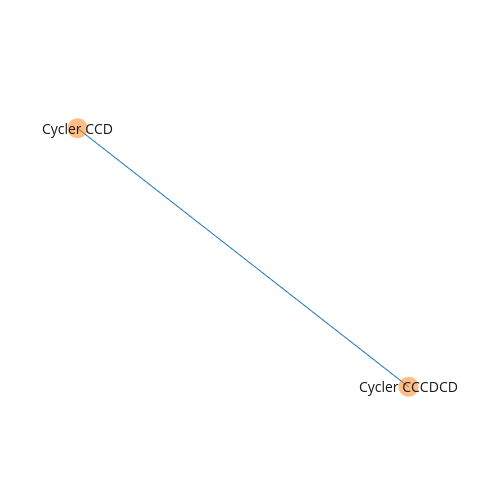
\includegraphics[width = 0.3\textwidth]{../img/neighbourhoods/12.png}} \\
% \end{figure}
% \begin{figure}[htbp!]
% \ContinuedFloat
% \subfloat[]{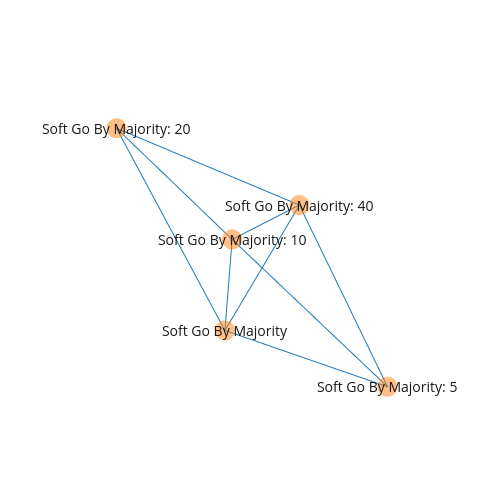
\includegraphics[width = 0.3\textwidth]{../img/neighbourhoods/13.png}}
% \subfloat[]{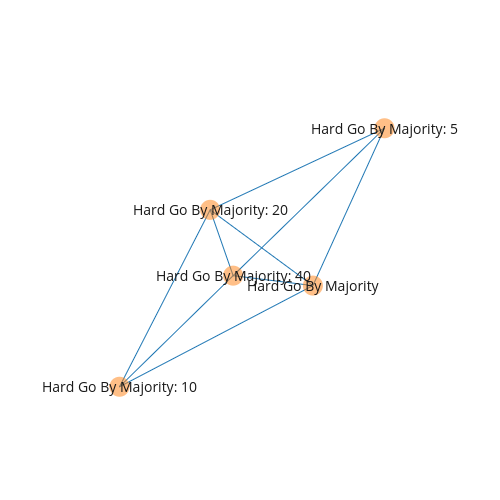
\includegraphics[width = 0.3\textwidth]{../img/neighbourhoods/14.png}}
% \subfloat[]{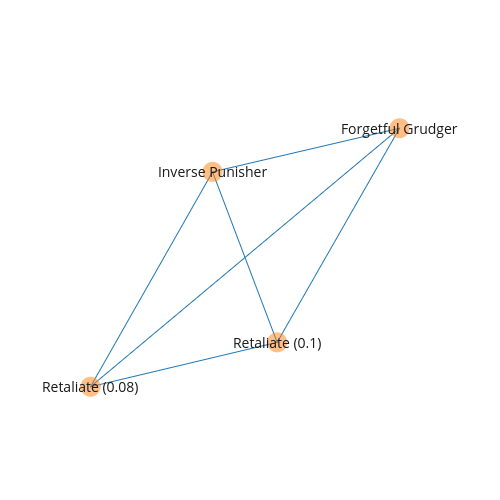
\includegraphics[width = 0.3\textwidth]{../img/neighbourhoods/15.png}} \\
% \end{figure}
% \begin{figure}[htbp!]
% \ContinuedFloat
% \subfloat[]{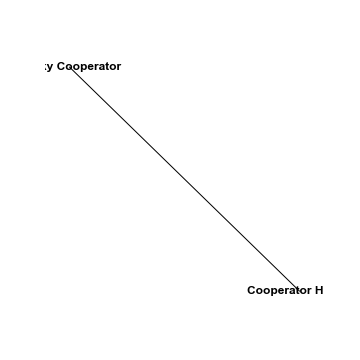
\includegraphics[width = 0.3\textwidth]{../img/neighbourhoods/16.png}}
% \subfloat[]{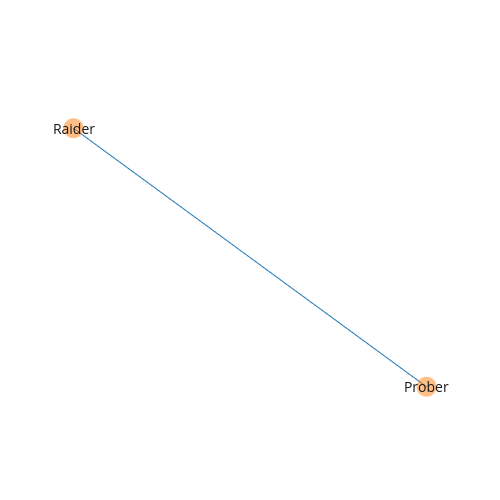
\includegraphics[width = 0.3\textwidth]{../img/neighbourhoods/17.png}}
% \subfloat[]{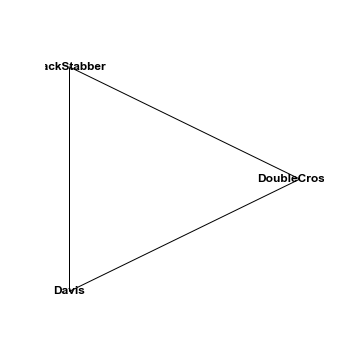
\includegraphics[width = 0.3\textwidth]{../img/neighbourhoods/18.png}} \\
% \end{figure}
% \begin{figure}[htbp!]
% \ContinuedFloat
% \subfloat[]{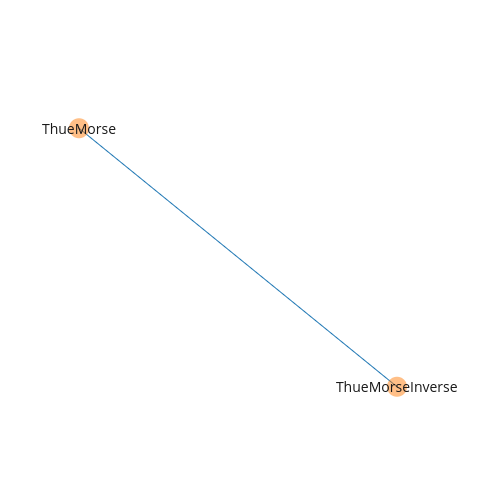
\includegraphics[width = 0.3\textwidth]{../img/neighbourhoods/19.png}}
% \subfloat[]{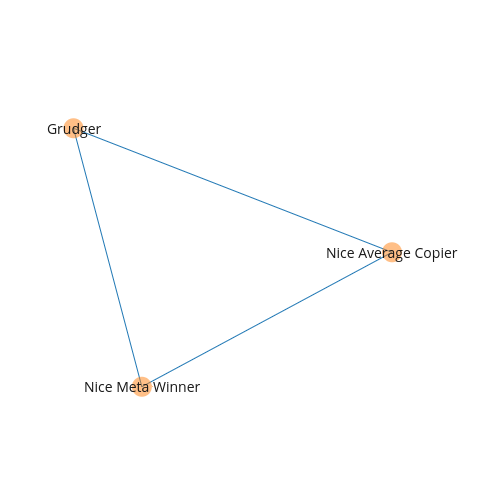
\includegraphics[width = 0.3\textwidth]{../img/neighbourhoods/20.png}}
% \subfloat[]{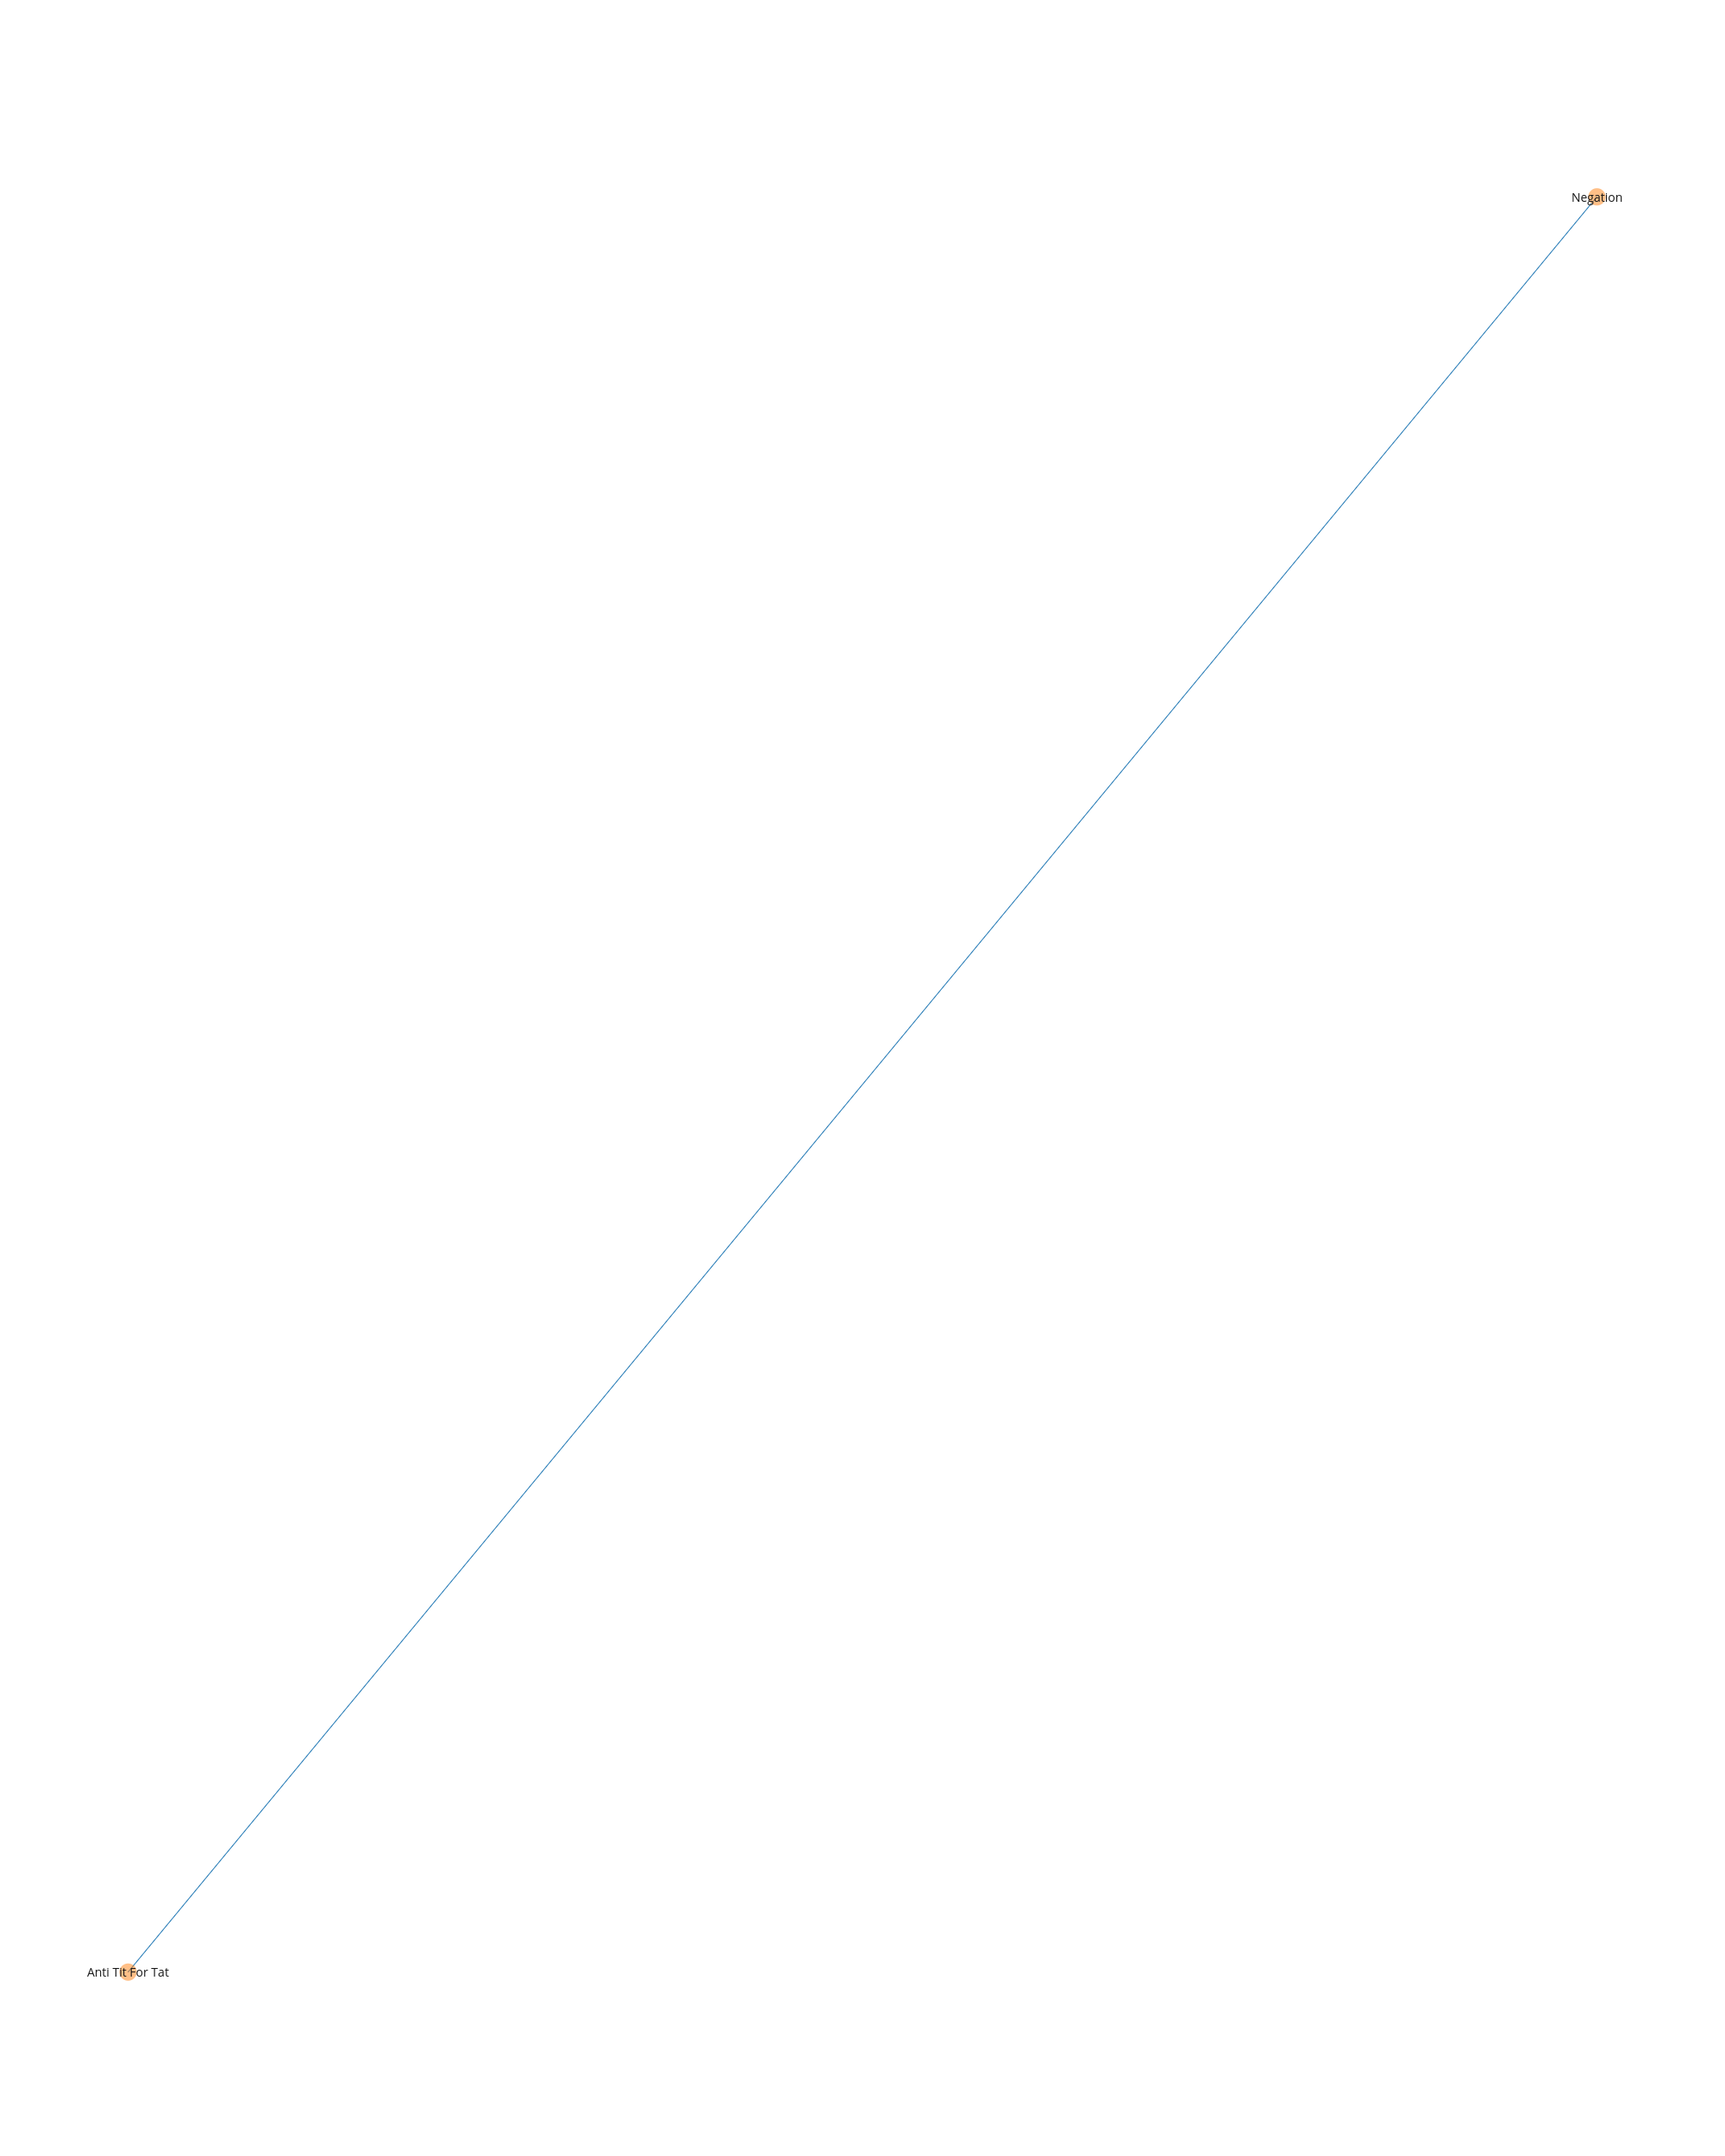
\includegraphics[width = 0.3\textwidth]{../img/neighbourhoods/21.png}} \\
% \end{figure}
% \begin{figure}[htbp!]
% \ContinuedFloat
% \subfloat[]{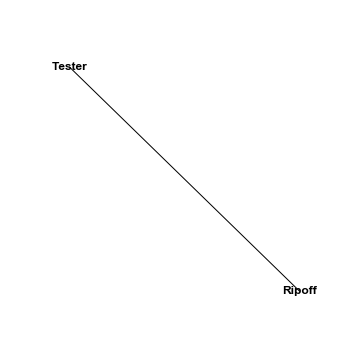
\includegraphics[width = 0.3\textwidth]{../img/neighbourhoods/22.png}}
% \subfloat[]{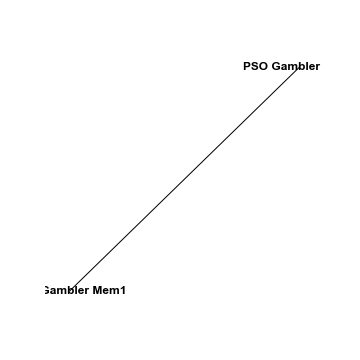
\includegraphics[width = 0.3\textwidth]{../img/neighbourhoods/23.png}}
% \subfloat[]{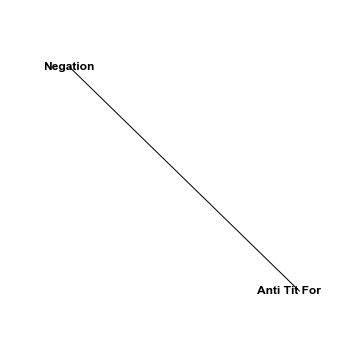
\includegraphics[width = 0.3\textwidth]{../img/neighbourhoods/24.png}} \\
% \end{figure}
% \begin{figure}[htbp!]
% \ContinuedFloat
% \subfloat[]{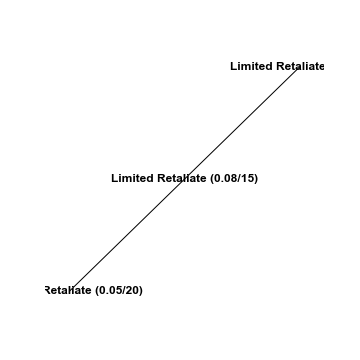
\includegraphics[width = 0.3\textwidth]{../img/neighbourhoods/25.png}}
% \subfloat[]{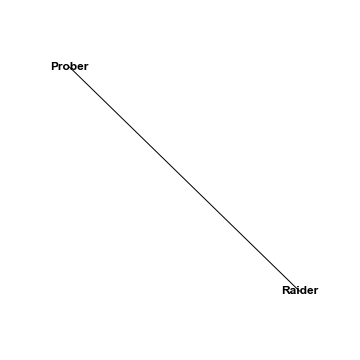
\includegraphics[width = 0.3\textwidth]{../img/neighbourhoods/0.png}}\\
% \end{figure}
